\documentclass[sigplan,review,anonymous]{acmart}\settopmatter{printfolios=true,printccs=false,printacmref=false}

\usepackage{xcolor}
\usepackage{amssymb} 
\usepackage{tikz}
\usepackage[autostyle]{csquotes}
\usepackage{listings}
\synctex=1

\usetikzlibrary{positioning}
\usetikzlibrary{arrows,automata}

\title{Handling String-Number Conversion in String Constraint Solving}
\author{}


%%%%%%%%%%%%%%%%%%%%%%%%%%%%%%%%%%%%%%%%%%%%%%%%%%%%%%%%%%%%%%%%%%%%%%%%%%%%%%
\begin{document}
%%%%%%%%%%%%%%%%%%%%%%%%%%%%%%%%%%%%%%%%%%%%%%%%%%%%%%%%%%%%%%%%%%%%%%%%%%%%%%
\newcommand{\hide}[1]{}

\newcommand{\todo}[1]{{\color{blue}TODO: #1}}
\newcommand{\lh}[1]{{\color{orange}Lukas: #1}}
\newcommand{\sti}[1]{\mbox{\textbf{toInt}($#1$)}}
\newcommand{\its}[1]{\mbox{\textbf{toStr}($#1$)}}
\newcommand{\varn}{\mbox{$\mathbb{V}_{\mathbb{Z}}$}}
\newcommand{\vars}{\mbox{$\mathbb{V}_{\Sigma^*}$}}
\newcommand{\cvar}{\mbox{$V_{\Sigma_\epsilon}$}}
\newcommand{\cvarone}{\mbox{$V^1_{\Sigma_\epsilon}$}}
\newcommand{\cvartwo}{\mbox{$V^2_{\Sigma_\epsilon}$}}
\newcommand{\modelof}[1]{[\![#1]\!]}
\newcommand{\true}{\mbox{$\mathsf{true}$}}
\newcommand{\false}{\mbox{$\mathsf{false}$}}
\newcommand{\enc}[1]{[\![#1]\!]}
\newcommand{\parikhof}[1]{\mathit{Parikh}{(#1)}}
\newcommand{\parikhwof}[2]{|#1|_{#2}}


\maketitle


\lstdefinelanguage{JavaScript}{
	keywords={typeof, new, true, false, catch, function, return, null, catch, switch, var, if, in, while, do, else, case, break},
	keywordstyle=\color{blue}\bfseries,
	ndkeywords={class, export, boolean, throw, implements, import, this},
	ndkeywordstyle=\color{darkgray}\bfseries,
	identifierstyle=\color{black},
	sensitive=false,
	comment=[l]{//},
	morecomment=[s]{/*}{*/},
	commentstyle=\color{purple}\ttfamily,
	stringstyle=\color{red}\ttfamily,
	morestring=[b]',
	morestring=[b]"
}





%%%%%%%%%%%%%%%%%%%%%%%%%%%%%%%%%%%%%%%%%%%%%%%%%%%%%%%%%%%%%%%%%%%%%%%%%%%%%%
\section{Introduction} \label{section:introduction}
%%%%%%%%%%%%%%%%%%%%%%%%%%%%%%%%%%%%%%%%%%%%%%%%%%%%%%%%%%%%%%%%%%%%%%%%%%%%%%



String constraint solving has received considerable attention in the constraint solving community, with solvers such as CVC4 and Z3 implmenting solvers of ever-increasing sophistication.  Operations such as substring and string length are widely supported, and recent solvers such as Z3-str3 have shown impressive results.  However, these solvers have limited for operations that convert between strings and integers; string length operations are sometimes well supported, but not parsing a string as an integer or turning an integer value into its string form.  When there is support, it is often limited to ground terms, i.e. at least one side of the conversion must be a constant.  Thus, $v = string2int("5")$ or $v = int2string(5)$ are handled but $v_1 = int2string(v_2)$ will fail.

As solvers such Z3 are applied to symbolic execution of programming languages, this is increasingly becoming a severe limitation.  For many languages such as Java, conversion between integers and strings is a niche operation, and much symbolic execution can be done without supporting it; however, this is not true of some scripting languages, of which JavaScript is the most notable.  JavaScript is a key language---it powers most interactive content on the Web, and increasingly server-side code with nodejs---and it has conversions between strings and integers embedded in the core of its semantics.

\begin{verbatim}
function resetArray(arr) {
  for(var i = 0; i < arr.length; i++) {
    arr[i] = 0
  }
}
\end{verbatim}



A casual glance at the above code reveal no use of strings at all, but the semantics of field access is somewhat unusual in JavaScript: all array indices act like strings, and numeric indices are converted to strings.  Any faithful symbolic execution of JavaScript must handle such conversions for even basic array operations to work correctly; consider the following code snippet that uses {\tt{resetArray}}, with the value of {\tt{x}} shown on the right:

\begin{tabular}{l|c}
	{\tt{x = [0, 1, 2, 3, 4, 5]}} & [0, 1, 2, 3, 4, 5] \\
	{\tt{resetArray(x)}} & [0, 0, 0, 0, 0, 0] \\
	{\tt{x["3"] = 5}} & [0, 0, 0, 5, 0, 0] \\
	{\tt{x["12"] = 7}} & [0, 0, 0, 5, 0, 0, , , , , , 7] \\
	{\tt{resetArray(x)}} & [0, 0, 0, 0, 0, 0, 0, 0, 0, 0, 0, 0] \\
\end{tabular}

In this code, string and integer values access the same array elements interchangeably, necessitating conversions between string and integers to faithfully model JavaScript semantics.  This conversion is mandated explicitly by JavaScript semantics: the 2019 edition of ECMAScript requires that $ToPropertyKey$ be called on the element expression (\S{12.3.2.1}), and $ToPropertyKey$ calls {\tt{ToString}} on that value in all but special cases (\S{7.1.14}).

Now observe that {\tt{resetArray}} assigns to the array in a loop of which the size cannot, in general, be known a priori; as such, falls into the case where neither the string nor the integer in a conversion are constant and hence most SMT solvers will not be able to handle it.  But this is a rather straightforward array operation, and so this limit will cripple any model of non-trivial JavaScript code.


\todo{The end of Julian's current writing}


\hide{Why this problem is important? Need to say it is used often, e.g., read 
from text file or user input. Why this problem is challenging? It is undecidable. Some tricky cases 
using string as array index. Bounded SAT-based encoding might not work even for 
very simple constraints. e.g., $y=str2int(x) \wedge y>9999999$, if $x$ is a 
ASCII string, then XXX Boolean variables are required. Or we can just propose 
an example that all major solver fails. Maybe we still say our approach is still over-approximation + under-approximation, in this case, need to think how to present the over-approximation part. Maybe no CEGAR is fine.}

String data type is omnipresent in modern programming languages. Various infamous security vulnerabilities such as injection and cross-site scripting attack are caused by malicious string values. As a results, in the past, a significant amount of research efforts have been investigated to symbolic execution and test case generation of string manipulating programs~\cite{saxena2010symbolic,artzi2011framework,huang2004securing,sen2013jalangi}. The core enabling technology for these approaches is string constraint solving~\cite{kiezun2009hampi,abdulla2014string,zheng2013z3,abdulla2015norn,abdulla2017flatten,wang2016string,abdulla2018trau,chen2019decision,zheng2017z3str2}. However, all these modern solvers fall short when \textit{string-number conversion function} occurs in the program.


String-number conversion function is very frequently used in string-manipulating programs. For example, often that programs read plain string input from text files, partition it according to some predefined separator symbol (e.g., the comma symbol), and then convert each string partition to the desired data type (often integers). In the reverse direction, programs also convert values in numerical data type back to string and store them as text files. 

Incorrect handling of string-number conversion can cause very subtle bugs.
For example, in JavaScript, variables are untyped and (implicit) type conversion happens automatically to the stored values. Consider the following simple program


\begin{lstlisting}[breaklines=true,language=JavaScript]
var arr = [1,...,M];
var input = //from user
if(0<=input<M-1){
	document.write(arr[input])
}
\end{lstlisting}

The program reads input value from users and use it as the array index. This program works perfectly no matter the input is in string form (e.g., ``1'', ``3'') or numerical form (e.g., $1$, $3$). Both of them can pass though the range test (when the input is a string, it will be first convert to integer and then compared with $0$ and $M$). However, the programmer may find later that he wants to shift the index value by one, say, change \texttt{document.write(arr[input])} to \texttt{document.write(arr[input+1])}. In such case, the program is still correct if \texttt{input} is a number, but will behave incorrectly if \texttt{input} is a string. For example, when \texttt{input=="5"}, the \texttt{+} operator in \texttt{input+1} will be interpreted as string concatenation and the value $1$ will be converted to a string. Therefore, the program will output \texttt{arr["51"]} instead of \texttt{arr["6"]}. If one searches CVE (Common Vulnerabilities and Exposures), he/she can find a number of vulnerabilities (e.g., clauses array-out-of-bound) due to incorrect handling of string-number conversion.

In the example above, we can detect the array-out-of-bound problem (that happens when \texttt{input} is a string) by checking the satisfiability of the string constraint below\footnote{The case \texttt{input} stores a integer value can be check by another formula.}. 

$$
\begin{array}{c}
0 \leq \sti{input}<M-1 \wedge \\
\neg(index = input\cdot \its{1} \wedge 0 \leq \sti{index} <M-1)
\end{array}
$$


Such constraint contains \textit{string-number conversion} functions (e.g., $\sti{input}$ and $\sti{index}$), \textit{equality constraints} (e.g., $index = input\cdot \its{1}$), and \textit{integer constraints} (e.g., $0 \leq \sti{input}<M$). Solving constraint of this kind is a very challenging problem. From the theoretical point of view, this problem is already proven to be undecidable~\cite{day2018satisfiability}. In practice, in our experiments, all of the state-of-the-art string constraint solvers do not support string-number conversion correctly. Some of them handles such constraints with only over-approximation of the original formula, and is known to have one-side error (see Section~\ref{section:evaluation} for detailed explanation). 
In this paper, we propose a framework that handles string constraints with string-number conversion efficiently. Our framework uses both over and under-approximation of the string constraints. The over-approximation is for proving UNSAT and the under-approximation is for proving SAT of the string constraint. Both over and under-approximation should fail in a decidable fragment of string constraints that can be efficiently solved. 

For over-approximation, there are a few existing algorithms~\cite{parosh2019chain,z3}, our framework does not set any restriction on which algorithm to be used. In our experiences, the UNSAT instances in all available benchmarks are not that difficult and many approaches can handle all of them almost perfectly. The battle field is in fact those SAT instances. 
In our prototype tool, we implement the algorithm presented in~\cite{parosh2019chain}, in addition with some additional axioms, to handle the over-approximation of string constraints with number-string conversion. 

For under-approximation, we restrict the search space of each string variable to strings that obey some predefined and parameterized pattern. By adjusting the parameters, one can easily enlarge or prune out the potential solution space. In paper, we propose to use patterns defined by \emph{symbolic flat automata} (SFA). The approach based on SFA is very flexible yet allows very efficiently manipulation. One can pick SFA of arbitrary structure for the search space restriction and reduce the string constraint solving problem to an integer constraint solving problem. For efficiency, it avoids the alphabet 
explosion problem that the approach in~\cite{abdulla2017flatten} suffers.

Based on the SFA encoding, we manage to translate the string constraint with string-number function to an equisatisfiable pure numerical constraints. Thus the problem is significantly simplified. We show that if we restrict the variable to arbitrary symbolic flat automata, one can convert the a string constraint with string-number function to an integer constraint consisting of both polynomials and exponentials. Solving such kind of constraints is a very difficult task. For simpler cases where the variables are real numbers, decision procedures for different subclass polynomial-exponential equations exists~\cite{gan2015decidability,kincaid2019closed,achatz2008deciding}. To the best of our knowledge, the satisfiability problem of polynomial-exponential equations is still open. For efficiency reason, we propose to use \emph{SFA with only one loop} to handle string-number conversion function. That is, if we encountered a constraint $y=\sti{x}$, then we always restrict the domain of $x$ to some SFA with one loop, instead of arbitrary SFAs. This allows us to convert a string constraint with string-number conversion function to a equisatisfiable linear integer constraint, which can be solved very efficiently. 

\todo{Talk about experiments}


To ease presentation, in the paper, we only consider string constraints consisting of \emph{equality constraints (a.k.a. word equation)}, \emph{length constraints}, and \emph{string-number conversion} functions. In fact, the approach can be easily extended to support transducer and membership constraints. The extension is implemented in our prototype tool \textsf{z3-Trau}. 


\hide{
suggest restricting the string domain to $0^*[0-9]^k$, where $k$ is the maximum 
digit allowed in the corresponding number value. In programming languages 
such  as JavaScript or Python, a number with $k$ digits can be converted from a 
string of length arbitrarily longer than $k$. For example, $12 = 
str2int(``0000012")$. That is why we use $0^*$ at the beginning of the pattern.
Under this domain, we can convert the string-number conversion constraints to 
linear integer constraints, which is much easier to solve. In our experience, 
usually, it suffices to find a solution using a small $k$ for a satisfiable 
constraint. Note that a 64-bit integer number corresponds to a string with 
$k\leq 21$.

Given a formula that is a boolean combination of different types of string constraints, e.g., $\phi=(|x| = |y| \vee \sti{x} = \sti{y})\wedge x = y$, an SMT solver based on the DPLL(T) algorithm~\cite{} treats each string constraint $|x| = |y|$, $\sti{x} = \sti{y}$, $xy=yx$ as a boolean variable, and systematically guesses possible solutions without considering their semantics as string constraints. E.g., the solver may guess $\neg(|x| = |y|)$, $(\sti{x} = \sti{y})$, and $(x =y)$. This is a valid guess if all the string constraints are just interpreted as boolean variables, but invalid when their semantics as string constraints are considered, because it cannot be the case that $x$ and $y$ are the same string $(x =y)$, but they are of different lengths $( \neg (|x| = |y|))$.


The approach combines techniques from both automata theory and SMT solving to explore the model space of a string constraint systematically. More specifically, an SMT solver based on the DPLL(T) algorithm~\cite{} is used to convert the satisfiability of a string constraint, which is an arbitrary boolean combination of string predicates, to the satisfiability problem of a set of string constraints in the form of conjunctions of string predicates.




}



%%%%%%%%%%%%%%%%%%%%%%%%%%%%%%%%%%%%%%%%%%%%%%%%%%%%%%%%%%%%%%%%%%%%%%%%%%%%%%
\section{Overview} \label{section:overview}
%%%%%%%%%%%%%%%%%%%%%%%%%%%%%%%%%%%%%%%%%%%%%%%%%%%%%%%%%%%%%%%%%%%%%%%%%%%%%%
For proving UNSAT, our strategy first over-approximates string-number conversion function $n=\its{x}$ as an uninterpreted function with an additional axiom $n\leq 0 \rightarrow \sti{\its{n}}=n$. 


and then solve the entire constraint with a procedure that is similar to the one in ATVA 2019.






%%%%%%%%%%%%%%%%%%%%%%%%%%%%%%%%%%%%%%%%%%%%%%%%%%%%%%%%%%%%%%%%%%%%%%%%%%%%%%
\section{Preliminaries} \label{section:preliminary}
%%%%%%%%%%%%%%%%%%%%%%%%%%%%%%%%%%%%%%%%%%%%%%%%%%%%%%%%%%%%%%%%%%%%%%%%%%%%%%
%We use $\mathbb{N}$ and $\mathbb{Z}$ to denote the sets of natural numbers and 
%integers. For a set $A$, we use $|A|$ to denote its size. For a string $w$, we 
%use $|w|$ to denote its length and $|w|_a$ to denote the number of occurrences of $a$ in $w$. We $\epsilon$ to denote an empty string and use $w_1\cdot w_2$ to denote the concatenation of strings $w_1$ and $w_2$. Let $S$ be a finite set of symbols. We use $S^+$ to denote the set of string over $S$ and $S^* = S^+\cup \{\epsilon\}$. We define $S_\epsilon =S\cup\{\epsilon\}$. A language 
%$L$ over $S$ is a set of strings in $S^*$. 
%
%A \emph{finite automaton} is a tuple $(Q,T,\Sigma,q_0,q_m)$, where $Q$ is the set of states, $T\subseteq Q\times (\Sigma\cup \{\epsilon\} )\times Q $ is the set of transition relation, $\Sigma$ is the alphabet, $q_0$ is the initial state, and $q_m$ is the final state. The semantics of finite automaton is defined in the standard manner. We use $L(A)$ to denote the regular language, i.e., set of accepted strings, of the automaton $A$.

%Given a finite automaton $A$ over $\{a_1,a_2,\ldots,a_n\}$, the Parikh image of $L$ is the set $\{(|w|_{a_1},\ldots, |w|_{a_n}) \mid w \in  L(A) \}$, i.e., the number of occurrences of each symbol $\{a_1,a_2,\ldots,a_n\}$ of words in $L(A)$. Moreover, one can construct from $A$ in linear time a Presburger formula $\phi_A(v_1, \ldots,v_n)$ such that $\phi(c_1, \ldots,c_n) \iff (c_1, \ldots,c_n)$ in the Parikh image of $L$~\cite{SeidlSMH04}.

We use $\mathbb{N}$ and $\mathbb{Z}$ to denote the sets of natural numbers (including 0) and 
integers. For a set $A$, we use $|A|$ to denote its size. 
An \emph{alphabet} is a finite set $\Sigma$ of \emph{characters} and a \emph{string} over $\Sigma$ is a sequence $w = a_1\ldots a_n$ of characters from $\Sigma$, with $\epsilon$ denoting the \emph{empty string}. 
We use $w_1\cdot w_2$ to denote the \emph{concatenation} of strings $w_1$ and $w_2$.
$\Sigma^*$ is the set of all strings over $\Sigma$, $\Sigma^+ = \Sigma^*\setminus \{\epsilon\}$, and 
A \emph{language} over $\Sigma$ is a subset $L$ of $\Sigma^*$.  
%
We use $|w|$ to denote the lenght of $w$ and $|w|_a$ to denote the number of occurrences of the character $a\in \Sigma$ in $w$.  
The \emph{Parikh image} of $w$ is the assignment 
%$\parikh(w) = \{a_1 \mapsto |w|_{a_1},\ldots, a_n \mapsto |w|_{a_n}\}$ that maps every symbol in $w$ to the number of its occurences in $w$. 
$\parikhof w$ that maps every character $a\in\Sigma$ to the number of its occurences in $w$, i.e., $\parikhof w (a) = |w|_a$. 
The Parikh image of a language $L$ is the set of Parikh images $\parikhof L = \{\parikhof w \mid w \in  L\}$. 

A \emph{finite automaton} is a tuple $(Q,T,\Sigma,q_0,q_m)$, where $Q$ is the set of \emph{states}, $T\subseteq Q\times (\Sigma\cup \{\epsilon\} )\times Q $ is the set of \emph{transitions}, $\Sigma$ is the alphabet, $q_0$ is the \emph{initial state}, and $q_m$ is the \emph{final state}. 
%The semantics of finite automaton is defined in the standard manner. 
We use $L(A)$ to denote the language of the automaton $A$, i.e., the set of accepted strings, defined in the standard manner.
\lh{If we later start technical talking about tings like runs then we should include this definition.}

 


%%%%%%%%%%%%%%%%%%%%%%%%%%%%%%%%%%%%%%%%%%%%%%%%%%%%%%%%%%%%%%%%%%%%%%%%%%%%%%
\section{String Constraints} \label{section:sc}
%%%%%%%%%%%%%%%%%%%%%%%%%%%%%%%%%%%%%%%%%%%%%%%%%%%%%%%%%%%%%%%%%%%%%%%%%%%%%%


In this section, we formally define string constraints. To begin with, we fix an finite alphabet $\Sigma \subseteq \mathbb{N}$. Note that here we assume the alphabet is a finite subset of natural numbers. Essentially, we try to capture the numerical encoding of the corresponding symbols in computers (e.g., in ASCII, `A' is encoded as $65$). We assume there is an one-one mapping between numbers in $\Sigma$ and the character it encodes. For the simplicity of presentation, we assume the character `$0$' is mapped to the number $0$, `$1$' to $1$,$\ldots$, and `$9$' to $9$. For other character $c$, we use $\enc{c}$ to denote the number that it maps to. Notice that this approach is general enough to support any finite set of characters. We write $[n,m]$ for the set of numbers (or symbols in $\Sigma$) $\{k\mid n\leq k \leq m\}$. 


We call $\vars$ the set of \emph{string variables} ranging over $\Sigma^*$ and $\varn$ the set of \emph{integer variables} ranging over $\mathbb{Z}$.
For a variable $x$, we call its primed version (e.g., $x'$) or indexed versions (e.g., $x_1$) its \emph{variants}.
In this paper, we use $x,y$ (or their variants) to denote string variables and $n$ (or its variants) to denote integer variables.

An \emph{interpretation over $\vars$ and $\varn$} is a mapping $I$ from $\vars\cup \varn$ to $\Sigma^* \cup \mathbb{N}$. A \emph{term} is an element in $(\vars\cup \Sigma)^*$. We lift the interpretation $I$ to terms and linear constraints in the standard manner. 

An \emph{equality constraint} $\phi_e$ is of the form $t_1 = t_2$ where $t_1, 
t_2$ are terms in $(\vars\cup \Sigma)^*$. The \emph{model} of $\phi_e$ is the set of interpretations $\modelof{\phi_e}=\{I\mid 
I(t_1)=I(t_2)\}$. A \emph{disequality constraint} is of the form $t_1 \neq 
t_2$ and is interpreted analogously.

An \emph{integer constraint} $\phi_i$ is a linear constraint over the variables in $\varn$ and length of a string $|x|$ for all $x \in \vars$.
%Formally, assume that $\vars=\{x_i,\ldots,x_n\}$ and $\varn=\{y_i,\ldots,y_m\}$, a length constraint is of the form $(\sum_{i\in[1,n]}(j_i \times \sti{x_i}+k_i\times |x_i|)+ \sum_{i\in[1,m]}(l_i \times y_i)) \odot k$, where $\odot \in \{>,\geq, =, \leq, <\}$, and $j_i,k_i,l_i,k\in \mathbb{Z}$. We define $\modelof{\phi}= \{I \mid (\sum_{i\in[1,n]}(j_i \times \sti{I(x_i)}+k_i\times |I(x_i)|)+ \sum_{i\in[1,m]}(l_i \times I(y_i))) \odot k \}$.
We define  $\modelof{\phi_i}= \{I \mid I(\phi_i)= \true \}$.

The \emph{string-number conversion constraint} $\phi_s$ is of the form $n=\sti{x}$, where the function $\sti{x}$ is defined as follows. For $a\in [0,9]$, we have $\sti{a}=a$ and for $s \cdot a \in [0,9]^+$, $\sti{s\cdot a} = 10\times \sti{s}+a$. For $s\notin [0,9]^+$, $\sti{s}=-1$. We define  $\modelof{\phi_s}= \{I \mid I(n)= \sti{I(x)} \}$.

A \emph{string constraint} $\phi$ is in the form of $\bigwedge_{\pi \in \Pi} \pi$, where $\Pi$ is a set of the above three kinds of constraints. We say that $\phi$ is \emph{satisfiable}  iff $\bigcap_{\pi \in \Pi} \modelof{\pi}$ is not empty.

Notice that only positive integer is supported in the string-number conversion function. This is the semantics used by most of the SMT solvers, and hence we follow it in this paper. The encoding has a benefit that it can also handle the case where $x$ is ``not a number'', using the condition $\sti{x} = -1$.

Supporting only positive integer is not a strong restriction, since conversing from negative integer can still be encoded using the positive only version. More specifically, if we want to say $n \in \varn$ is the integer value of the string $x \in \Sigma^*$, we can write the following constraint (ignore the case that $x$ is ``not a number'', which can also be encoded using more conditions):
$$(n= \sti{x}) \vee (n=-\sti{x'} \wedge x = \enc{-}\cdot x')$$
Recall that $\enc{-}$ is the integer encoding of the minus symbol `$-$'. The \emph{number-string conversion function} $\its{n}$ is defined symmetrically. We have $x = \its{n}$ iff $y= \sti{n}$. 




%%%%%%%%%%%%%%%%%%%%%%%%%%%%%%%%%%%%%%%%%%%%%%%%%%%%%%%%%%%%%%%%%%%%%%%%%%%%%%
\section{Symbolic Flat Automata} \label{section:sfa}
%%%%%%%%%%%%%%%%%%%%%%%%%%%%%%%%%%%%%%%%%%%%%%%%%%%%%%%%%%%%%%%%%%%%%%%%%%%%%%
\newcommand{\st}[2]{q_{#1}^{#2}}
\newcommand{\sym}[2]{v_{#1}^{#2}}
%We use $\cvar$ to denote a finite set of \emph{character variables}  ranging over $\Sigma_\epsilon$. 
%Sometimes we use index to denote different set of variables over the same range, e.g., $\cvarone$ and $\cvartwo$. 
%We use $v$ and its variants for character variables. We call a string over $\cvar$ (character variables) a \emph{symbolic string}.
%An \emph{interpretation $I$ over $\cvar$} is a mapping from $\cvar$ to $\Sigma_\epsilon$. For a symbolic string $x= v_1v_2\cdots v_k$ over $\cvar$, $I(x)$ is defined as $I(v_1)\cdot I(v_2)\cdot \ldots \cdot I(v_k)$.

We introduce \emph{symbolic flat automata} (SFA) that will be used to define patterns 
%for the string variable domain restriction. 
used by the underapproximation module to restrict the domain of string variables. 
Namely, an SFA is a finite automaton $A = (Q,T,\cvar,\st{0}{0},\st{m}{0})$ operating over the alphabet $\cvar$ of \emph{character variables}, 
and satisfying the following structural constraints:
\begin{enumerate}
	\item The final state $\st{m}{0}$ is reached from  the initial state $\st{0}{0}$ through a stright path of $m-1$ transitions $(\st{i}{0},v_i,\st{i+1}{0}) \in T$, $\st{i}{0} \in Q$ for $i\in[0,m-1]$. %, with pairwise distiand states $\st{i}{0} \in Q$ for $i\in[0,m-1]$.
	\item  
Each state $\st{i}{0}$ is the origin of a unique simple cycle of the length $l_i\in\mathbb{N}$, consisting of states $\st{i}{j} \in Q$ and transitions $(\st{i}{j-1}, \sym{i}{j-1}, \st{i}{j \bmod l_i})$ for $j\in [1,l_i]$. 
Notice that case when $l_i = 0$ is also admissible and means that there is no cycle on $q_i$.
%Assume that $\st{i}{0}$ is included in a cycle with $l_i$ states (includes $\st{i}{0}$). 
%For each $j\in [1,l_i]$, we have $\st{i}{j} \in Q$ and $(\st{i}{j-1}, \sym{i}{j-1}, \st{i}{j \bmod l_i})$. 
%(where $l_i = 0$ means that there is no cycle on $q_i$)
	\item Each variable in $\cvar$ appears on at most one transition (but $\epsilon$ transition can appear multiple times). 
\end{enumerate} 
%Such automata are recognizers of symbolic strings, i.e., strings over $\cvar$.
Symbolic automata accept strings over $\cvar$, called \emph{symbolic strings}. 
Each symbolic string may be interpeted as a string over $\Sigma$, given an assignment of characters to its character variables.  
%
Formally, an \emph{interpretation $I$ over $\cvar$} is a mapping from $\cvar$ to $\Sigma_\epsilon$ and for a symbolic string $x= v_1v_2\cdots v_k$ over $\cvar$, $I(x)$ is defined as $I(v_1)\cdot I(v_2)\cdot \ldots \cdot I(v_k)$. 

\begin{figure*}
	\tikzset{state/.style={circle,draw=blue!50,fill=blue!20,
			thick,inner sep=0pt,minimum size=6mm}, initial text=$ $}
	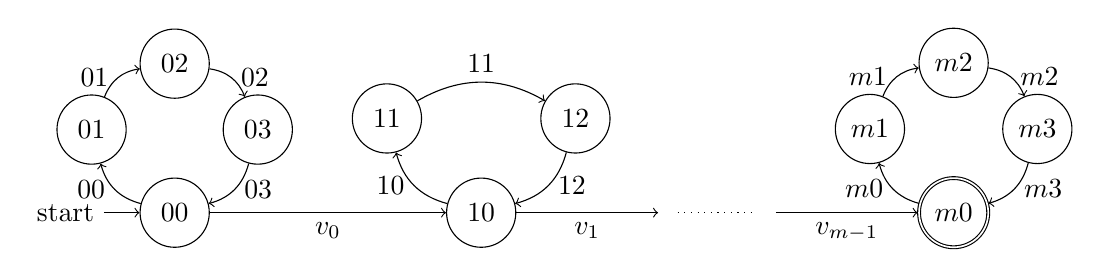
\begin{tikzpicture} 
		\node[state,initial] (q0)  {$\st{0}{0}$};
		\node[state] (q1) [right = 3cm of q0] {$\st{1}{0}$};
		\node (q2) [right = 1.8cm of q1]{};
		\node (q3) [right = 1cm of q2]{};
		\node[state,accepting] (qm) [right = 1.8cm of q3] {$\st{m}{0}$};
		
		\node[state] (q01) [above left = 0.6cm of q0] {$\st{0}{1}$};
		\node[state] (q02) [above = 1cm of q0] {$\st{0}{2}$};
		\node[state] (q03) [above right = 0.6cm of q0] {$\st{0}{3}$};

		\node[state] (q11) [above left = 0.8cm of q1] {$\st{1}{1}$};
		\node[state] (q12) [above right = 0.8cm of q1] {$\st{1}{2}$};

		\node[state] (qm1) [above left = 0.6cm of qm] {$\st{m}{1}$};
		\node[state] (qm2) [above = 1cm of qm] {$\st{m}{2}$};
		\node[state] (qm3) [above right = 0.6cm of qm] {$\st{m}{3}$};

  		\draw[->] (q0) edge [bend left] node [left]{$\sym{0}{0}$} (q01) ;
  		\draw[->] (q01) edge [bend left] node [left]{$\sym{0}{1}$} (q02) ;
  		\draw[->] (q02) edge [bend left] node [right]{$\sym{0}{2}$} (q03) ;
  		\draw[->] (q03) edge [bend left] node [right]{$\sym{0}{3}$} (q0) ;
  		
  		\draw[->] (q0) edge node [below]{$v_0$} (q1) ;
  		\draw[->] (q1) edge node [below]{$v_1$} (q2) ;
  		\draw[dotted] (q2) edge (q3) ;
  		\draw[->] (q3) edge node [below]{$v_{m-1}$} (qm) ;

  		\draw[->] (qm) edge [bend left] node [left]{$\sym{m}{0}$} (qm1) ;
		\draw[->] (qm1) edge [bend left] node [left]{$\sym{m}{1}$} (qm2) ;
		\draw[->] (qm2) edge [bend left] node [right]{$\sym{m}{2}$} (qm3) ;
		\draw[->] (qm3) edge [bend left] node [right]{$\sym{m}{3}$} (qm) ;

  		\draw[->] (q1) edge [bend left] node [left]{$\sym{1}{0}$} (q11) ;
		\draw[->] (q11) edge [bend left] node [above]{$\sym{1}{1}$} (q12) ;
		\draw[->] (q12) edge [bend left] node [right]{$\sym{1}{2}$} (q1) ;
	\end{tikzpicture} 

	\caption{An example of a symbolic flat automaton}
	\label{fig:sfa_def}
\end{figure*}

%A finite automaton $D=(Q,T',\Sigma,q_0,q_m)$ is an \emph{instance} of a SFA $S=(Q,T,\cvar,q_0,q_m)$, if there exists an interpretation $I: \cvar \cup \{\epsilon\} \rightarrow \Sigma_\epsilon$ satisfying $I(\epsilon)=\epsilon$ and $T'=\{(q,I(c),q')\mid (q,c,q')\in T\}$. We write $I(S)$ to denote the instance of $S$ wrt. $I$. The language of $S$ is defined as $L(S)= \cup\{L(D) \mid D \mbox{ is an instance of } S\}$. Notice that $L(S)$ is regular because every SFA has only finitely many instance and the finite union of regular languages are also regular.

The purpose of the structural restrictions of SFA is to ensure that the words of $L(A)$ are uniquely determined by their Parikh images, as formalised by the following lemma.  

\begin{lemma}
%Distinct words from the language of an SFA must have distinct Parikh images.  
For an SFA $A$ and $x,y\in L(A)$ if $\parikhof x = \parikhof y$ then $x = y$. 
%Distict words from the language of an SFA have distinct Parikh images.  
\end{lemma}
Indeed, notice that each accepted symbolic string $x$ is determined by the numbers of repetitions of individual cycles in the accepting run of $A$ over $x$.
Since every variable appears on at most one transition, then the $\parikhof x$ value of all variables appearing within the same cycle is the same, and it is equal to the number of repetitions of that cycle in the accepting run. 
%
The accepting run on $x$ (and so $x$ itself) can thus be reconstructed from $\parikhof x$.

For example, in the example of Figure~\ref{fig:sfa_def}, 
from $\parikhwof x {v_0} = \parikhwof x {v_1} = \cdots = \parikhwof x {v_{m-1}}=1$ and $\parikhwof x {v^0_1}=\parikhwof x {v^1_1}=\parikhwof x {v^2_1}=2$ we derive that $x=v_0(v^0_1v^1_1v^2_1)^2v_1\cdots v_{m-1}$. 
\todo{add Presburger constraints to allow more expressive power.}

%For such kind of automata, the number of occurrence of each symbol in $\cvar$ uniquely characterize an accepting symbolic string. For example, in the example of Figure~\ref{fig:sfa_def}, if the string $v_0(v^0_1v^1_1v^2_1)^2v_1v_{m-1}$ is accepted, then all other strings $w$ with $|w|_{v_0}=|w|_{v_1}=\ldots=|w|_{v_{m-1}}=1$ and also $|w|_{v^0_1}=|w|_{v^1_1}=|w|_{v^2_1}=2$ are not accepted. Moreover, from $|w|_{v_0}=|w|_{v_1}=\ldots=|w|_{v_{m-1}}=1$ and $|w|_{v^0_1}=|w|_{v^1_1}=|w|_{v^2_1}=2$, we can derive $w=v_0(v^0_1v^1_1v^2_1)^2v_1v_{m-1}$ by exploring the automata structure. \todo{add Presburger constraints to allow more expressive power.}


\lh{so far not sure about how and where to present this:}
\begin{lemma}
	Symbolic flat automata are closed under concatenation.
\end{lemma}






%\section{Handling Equality and Disequality Constraint Symbolically} \label{section:eq}
\section{Flat Underapproximation for Equalities and Regular Constraints} \label{section:eq}

Given an equality constraint $x_1\cdot x_2 \cdots x_n = x_{n+1}\cdot x_{n+2} \cdots x_m$, we restrict the domain of all variables to some SFA with disjoint alphabet and then connect the final state and initial state of two consecutive variables with an epsilon transition. We rename the variables on the transitions of SFA's for different occurrences of the same variable in one equality constraint. Later we will use some arithmetic constraints to enforce that all occurrences of the variants of the same variable will be assigned the same value. For notational convenience, the renaming is done by adding a version number to the variable. For example, we can rename $v_1$ to $v_1^{(0)}$, $v_1^{(1)}$, $\ldots$.

For the constraint $xy = yx$, we first restrict the domains of $x$ and $y$ to the SFA in Figure~\ref{fig:sfa} (a) and (b), respectively. In the construction of the SFA for $xy$ and $yx$ (Figure~\ref{fig:sfa} (c) and (d)), we rename the variables on the SFA of $X$ and $Y$ to some fresh variable for each different occurrence of $x$ and $y$ in $xy = yx$.

\begin{figure*}
	\tikzset{state/.style={circle,draw=blue!50,fill=blue!20,
			thick,inner sep=0pt,minimum size=6mm}, initial text=$ $}
		
 	\begin{minipage}[t]{0.15\textwidth} 
	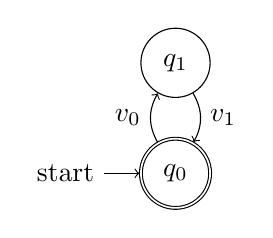
\begin{tikzpicture}
	\node[state,initial,accepting] (q0)  {$q_0$};
	
	\node[state] (q01) [above = 0.5cm of q0] {$q_1$};

	\draw[->] (q0) edge [bend left] node [left]{$v_0$} (q01) ;
	\draw[->] (q01) edge [bend left] node [right]{$v_1$} (q0) ;
	\end{tikzpicture} 
	
	\centering
	(a) $A_x$
	\end{minipage}
 	\begin{minipage}[t]{0.15\textwidth} 
	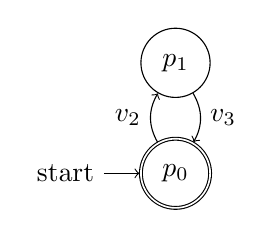
\begin{tikzpicture} 
	\node[state,initial,accepting] (q0)  {$p_0$};
	
	\node[state] (q01) [above = 0.5cm of q0] {$p_1$};
	
	\draw[->] (q0) edge [bend left] node [left]{$v_2$} (q01) ;
	\draw[->] (q01) edge [bend left] node [right]{$v_3$} (q0) ;
	\end{tikzpicture} 
	
	\centering
	(b) $A_y$
	\end{minipage}
	\begin{minipage}[t]{0.28\textwidth}
	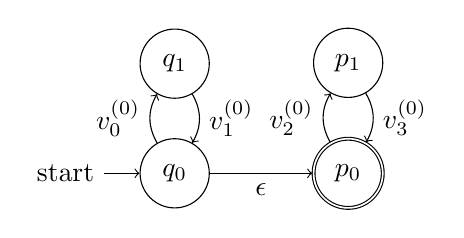
\begin{tikzpicture} 
	\node[state,initial] (q0)  {$q_0$};
	\node[state,accepting] (q1) [right = 1.3cm of q0] {$p_0$};
	
	\node[state] (q01) [above = 0.5cm of q0] {$q_1$};

	\draw[->] (q0) edge [bend left] node [left]{$v_0^{(0)}$} (q01) ;
	\draw[->] (q01) edge [bend left] node [right]{$v_1^{(0)}$} (q0) ;
	
	\node[state] (q11) [above = 0.5cm of q1] {$p_1$};
	
	\draw[->] (q1) edge [bend left] node [left]{$v_2^{(0)}$} (q11) ;
	\draw[->] (q11) edge [bend left] node [right]{$v_3^{(0)}$} (q1) ;
	\draw[->] (q0) edge  node [below]{$\epsilon$} (q1) ;
	\end{tikzpicture}
	
	\centering
	(c) $A_{xy}$
	\end{minipage}
	\ \ \ 
	\begin{minipage}[t]{0.28\textwidth}
	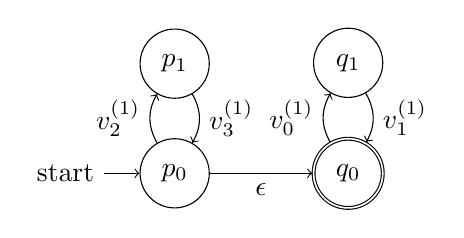
\begin{tikzpicture} 
	\node[state,accepting] (q0)  {$q_0$};
	\node[state,initial] (q1) [left = 1.3cm of q0] {$p_0$};
	
	\node[state] (q01) [above = 0.5cm of q0] {$q_1$};
	
	\draw[->] (q0) edge [bend left] node [left]{$v_0^{(1)}$} (q01) ;
	\draw[->] (q01) edge [bend left] node [right]{$v_1^{(1)}$} (q0) ;
	
	\node[state] (q11) [above = 0.5cm of q1] {$p_1$};
	
	\draw[->] (q1) edge [bend left] node [left]{$v_2^{(1)}$} (q11) ;
	\draw[->] (q11) edge [bend left] node [right]{$v_3^{(1)}$} (q1) ;
	\draw[->] (q1) edge  node [below]{$\epsilon$} (q0) ;
	\end{tikzpicture}
	
	\centering
	(d) $A_{yx}$
	\end{minipage}

	\caption{Symbolic flat automata of $x$, $y$, $xy$ and $yx$}
	\label{fig:sfa}
\end{figure*}

Assume that $S_n=(Q,T,\cvarone,q_i,q_f)$ is the SFA of $x_1\cdot x_2 \cdots x_n$ and $S_m=(P,T',\cvartwo,p_i,p_f)$ is the SFA of $x_{n+1}\cdot x_{n+2} \cdots x_m$. Our next task is to find a model for $x_1\cdot x_2 \cdots x_n = x_{n+1}\cdot x_{n+2} \cdots x_m$ under the domain restriction specified by $S_n$ and $S_m$. 
Note that $\cvarone \cap \cvartwo =\emptyset$, because all variables will be renamed to some fresh variable. 


This is equivalent to finding a pair of symbolic strings $(w_n,w_m) \in L(S_n)\times L(S_m)$ and a common interpretation $I$ such that 
\begin{enumerate}
	\item $I(w_n)=I(w_m)$
	\item $I$ assign to variants of the same variable the same value. For example, in Figure~\ref{fig:sfa} (c) and (d), $v_0^{(0)}$ and $v_0^{(1)}$ should be assigned the same value.
	\item different versions of the same variable should occurs equally often in $w_n\cdot w_m$. For example, in Figure~\ref{fig:sfa} (c) and (d), $w_{xy}=v_0^{(0)}v_1^{(0)}v_0^{(0)}v_1^{(0)}$ and $w_{yx}=v_0^{(1)}v_1^{(1)}v_0^{(1)}v_1^{(1)}$ is a pair of symbolic strings satisfying this condition. The number of occurrences of $v_i^{(0)}$ is the same to $v_i^{(1)}$ for $i\in[0,1]$ in the concatenation $w_{xy}\cdot w_{yx}$.
	But the pair $v_0^{(0)}v_1^{(0)}v_0^{(0)}v_1^{(0)}$ and $v_2^{(0)}v_3^{(0)}v_2^{(0)}v_3^{(0)}$ does not satisfy the condition. Observe that $v_0^{(0)}$ occurs twice, but $v_0^{(1)}$ is not there.
\end{enumerate}

In order to find such a pair of symbolic strings $(w_n,w_m) \in L(S_n)\times L(S_m)$ and an interpretation $I$, we first build a ``product'' automaton of $S_n$ and $S_m$ and then add some additional linear arithmetic constraints to enforce the above conditions.

Such product automaton uses $Q\times P$ as the set of states and $(\cvarone \cup \{\epsilon\}) \times (\cvartwo \cup \{\epsilon\} )$ as the alphabet. If a transition $((q_1,p_1), (v_i^{(j)},v_{i'}^{(j')}),(q_2,p_2))$ is taken, for some $i,j,i',j' \in \mathbb{N}$, it means the character variable $v_i$ and $v_{i'}$ (and so all of their indexed variants) should be assigned the same value and this value leads $S_n$ from state $q_1$ to state $q_2$ and $S_m$ from $p_1$ to $p_2$.

More precisely, the product automaton is a tuple $(Q\times P, T^2, (\cvarone \cup \{\epsilon\}) \times (\cvartwo \cup \{\epsilon\} ), (q_i,p_i),(q_f,p_f))$, where the transition relation $T^2$ is the minimal set satisfying the following.

\begin{itemize}
\item If $(q_1,v_i^{(j)},q_2) \in T$, then for all states $p\in P$, we have $((q_1,p),(v_i^{(j)},\epsilon),(q_2,p))\in T^2$.
\item If $(p_1,v_i^{(j)},p_2) \in T'$, then for all states $q\in Q,((q,p_1)$, we have $(\epsilon,v_i^{(j)}),(q,p_2))\in T^2$.
\item If $(q_1,v_i^{(j)},q_2) \in T$ and $(p_1,v_{i'}^{(j')},p_2) \in T'$, then we have $((q_1,p_1),(v_i^{(j)},v_{i'}^{(j')}),(q_2,p_2))\in T^2$.
\end{itemize}	
The first two cases correspond to the situation when the character variable $v_i^{(j)}$ is assigned $\epsilon$. In such cases, only one automaton changes its state.

For example, in the product automaton $A_{xy=yx}$ corresponds to $xy=yx$, we have the following transitions
\begin{itemize}
	\item $((q_0,p_0), (v_0^{(0)},\epsilon),(q_1,p_0))$, because $(q_0,v_0^{(0)},q_1)$ is a transition of $A_{xy}$.
	\item $((q_0,p_0), (\epsilon,\epsilon),(q_0,q_0))$, because $(p_0,\epsilon,q_0)$ is a transition of $A_{yx}$.
	\item $((q_0,p_0), (v_0^{(0)},v_2^{(1)}),(q_1,q_1))$, because $(q_0,v_0^{(0)},q_1)$ is a transition of $A_{xy}$ and $(p_0,v_2^{(1)},p_1)$ is a transition of $A_{yx}$.
\end{itemize}

Recall that for flat automata, the number of occurrences of each symbol uniquely characterizes an accepting string (Section~\ref{section:sfa}) and for any finite automaton we can construct a Presburger formula characterizing its Parikh image (Section~\ref{section:preliminary}). For a product automaton $A$ computed from the previous step, we compute a Presburger formula $\phi(A)$ over the set of variables $\{\#{(v_i^{(j)},v_{i'}^{(j')})}\mid (v_i^{(j)},v_{i'}^{(j')}) \in \cvarone \times \cvartwo\}$ characterizing the Parikh image of $A$. We use $\#(v_i)$ and $\#(v_i^{(j)})$ to denote the number of occurrences of $v_i$ and $v_i^{(j)}$, respectively. The following formulae establish the relation of the number of occurrences of symbols between the SFAs and the product automaton.
\begin{enumerate}
	\item for all $v_i^{(j)} \in \cvarone$, $\#(v_i^{(j)}) = \sum_{v \in {\cvartwo \cup \{\epsilon\}}} \#{(v_i^{j},v)}$   
	\item for all $v_i^{(j)} \in \cvartwo$, $\#(v_i^{(j)}) = \sum_{v \in {\cvarone \cup \{\epsilon\}}} \#{(v,v_i^{j})}$ 
\end{enumerate}

Then we add the following linear constraints to enforce  condition 1. and 2. required for the pair of symbolic string $(w_n, w_m)$ and $I$, i.e., $I(w_n) = I(w_m)$ and $I$ assign the same value to all versions of the same variable (we use $-1$ as the value of $\epsilon$). 
\begin{enumerate}
	\item for all $v_i^{(j)}\in \cvarone$ and $v_{i'}^{(j')}\in \cvartwo$, $\#{(v_i^{(j)},v_{i'}^{(j')})}>0 \rightarrow (v_i=v_{i'})$, 
	\item for all $v_i^{(j)}\in \cvarone$, $\#{(v_i^{(j)},\epsilon)}>0 \rightarrow (v_i=\epsilon)$, and
	\item for all $v_{i'}^{(j')}\in \cvartwo$,$\#{(\epsilon,v_{i'}^{(j')})}>0 \rightarrow (v_{i'}=\epsilon)$.
\end{enumerate}
We then add the linear constraints $\#(v_i) = \#(v_i^{(j)})$, for all $v_i\in \cvar$ and all different version numbers $j$ for $v_i$, to enforce condition 3, which says different versions of the same variable should occurs equally often in $w_n\cdot w_m$. 

From the model $M$ of the linear constraints, we can obtain $w_n$, $w_m$, and $I$. The interpretation $I$ is defined as $I(v)=M(v)$ for all $v\in (\cvarone \cup \cvartwo)$. The symbolic words $w_n$ and $w_m$ can be obtained by traverse the SFAs following the number of occurrences of each character variables.
More specifically, assume that the SFA $S_n$ is the one in Figure~\ref{fig:sfa_def}, then $$w_n = (v_0^0v_0^1v_0^2v_0^3)^{\#(v_0^0)}v_0(v_1^0v_1^1v_1^2)^{\#(v_1^0)}v_1\ldots(v_m^0v_m^1v_m^2v_m^3)^{\#(v_m^0)}$$
Note that $\#(v_0^0)=\#(v_0^1)=\#(v_0^2)=\#(v_0^3)$, so we just use $\#(v_0^0)$ to denote the number of times of first loop traversal. One can construct $w_m$ in a similar way. Using the same approach, one can derive the assignment to variables in $\vars$ using the corresponding count and values of variables in $\cvar$.

Disquality constraint $x_1\cdot x_2 \cdots x_n \neq x_{n+1}\cdot x_{n+2} \cdots x_m$ can be converted to equal-satisfiable equality constraints in the standard way~\cite{abdulla2015norn}. We replace it with the following constraints.

$$
\begin{array}{c}
(|x_1|+ |x_2|+ \cdots +|x_n| \neq |x_{n+1}| + |x_{n+2}|+ \cdots +|x_m|)\vee \\
\left(
	\begin{array}{cccc}
	
	 y_1\cdot y_2\cdot y_3 &=& x_1\cdot x_2 \cdots x_n &\wedge\\
	 y_1 \cdot y'_2 \cdot y'_3 &=& x_{n+1}\cdot x_{n+2} \cdots x_m &\wedge\\
	|y_2|&=&|y'_2|=1
	\end{array}

\right)
\end{array}
$$

The second disjunct says that the constraints $x_1\cdot x_2 \cdots x_n$ and $x_{n+1}\cdot x_{n+2} \cdots x_m$ have a common prefix $y_1$, but the next character $y_2$ and $y'_2$ is different. In an more efficient implementation, one just project $y_2$ and $y'_2$ to a SFA that accept only symbolic words $v_1$ and $v'_1$, respectively (the SFA has no loop and only one transition). 



\todo{Maybe talk about the heuristic that we merge the list elements into one}





%%%%%%%%%%%%%%%%%%%%%%%%%%%%%%%%%%%%%%%%%%%%%%%%%%%%%%%%%%%%%%%%%%%%%%%%%%%%%%
\section{Handling String-Integer Conversion} \label{section:s2i}
%%%%%%%%%%%%%%%%%%%%%%%%%%%%%%%%%%%%%%%%%%%%%%%%%%%%%%%%%%%%%%%%%%%%%%%%%%%%%%

In this section, we discuss how to handle the constraint $n=\sti{x}$ by restrict the domain of $x$ to some SFA. Let us begin with a simple example, assume that we use the SFA in Figure~\ref{fig:sfa} (a) to restrict the domain of $x$. Then we know that when $0\leq v_0,v_1 \leq 9$, then $n$ is a positive integer value, and otherwise $n =-1$. So we should first add the constraint $ ((0\leq v_0\leq 9) \wedge (0\leq v_1\leq 9)) \vee n=-1 $.

For the case that $n$ is a positive integer, the value of $n$ can be characterized by a constraint $n= (v_0\times 10+ v_1) \times (1+100 +100^2 + \ldots 100 ^{\#(v_0)-1})=  (v_0\times 10+ v_1) \times \frac{100^{\#(v_0)+1}-1}{100-1}$. 
The constraint uses $\#(v_0)$ to capture the total number of loop traversal.
Notice that the constraint above contains an exponential component $100^{\#(v_0)}$. To solve the satisfiability of this formula, one need to solve an exponential constraint. 

For a more general form, if we restrict the domain of $x$ to the SFA in Figure~\ref{fig:sfa} (c), for the case when $n$ is positive, we have the relation $n= (v_0^{(0)}\times 10+ v_1^{(0)}) \times (1+100 +100^2 + \ldots 100 ^{v_0^{(0)}-1})\times 100^{v_2^{(0)}}+(v_2^{(0)}\times 10+ v_3^{(0)}) \times (1+100 +100^2 + \ldots 100 ^{v_2^{(0)}-1}) =  (v_0^{(0)}\times 10+ v_1^{(0)}) \times \frac{100^{\#(v_0^{(0)})+1}-1}{100-1}\times 100^{v_2^{(0)}} + (v_2^{(0)}\times 10+ v_3^{(0)}) \times \frac{100^{\#(v_2^{(0)})+1}-1}{100-1}$. Observe that the formula has even more exponential components.

To the best of our knowledge, the satisfiability problem of integer constraints with a mix of polynomials and exponentials is still open. 

For the particular case with only one integer variable, the satisfiability of integer constraints with a mix of polynomials and exponentials can be decided using the algorithm in~\cite{POPL2019}. However, the algorithm involves a quantifier elimination procedure, which is double-exponential to the length of the input formula and hence cannot handle large instances. 

In order to handle the under-approximation of string-integer conversion efficiently, we propose to restrict the domain of $x$ to a SFA in Figure~\ref{fig:sfa_its}. 

The SFA has a self-loop transition labeled $v_0$ at $q_0$ and we always add a constraint $v_0=0$ for such SFA. With this transition, we can ensure that the under-approximation handles all numbers with at most $m$ digits. Notice that even for a bounded integer, the corresponding string can be of unbounded length with arbitrarily many `$0$' characters at the front. For example, the formula $\sti{x}=10 \wedge |x|=5$ is satisfiable when $x=``00010"$. 

\begin{figure}
	\tikzset{state/.style={circle,draw=blue!50,fill=blue!20,
			thick,inner sep=0pt,minimum size=6mm}, initial text=$ $}
	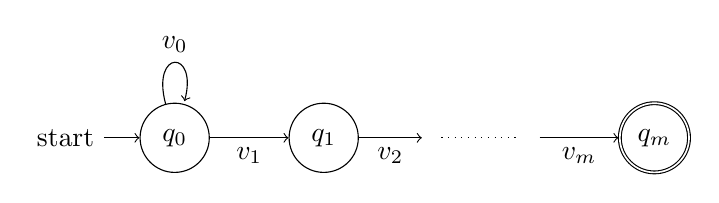
\begin{tikzpicture} 
	\node[state,initial] (q0)  {$q_0$};
	\node[state] (q1) [right = 1cm of q0] {$q_1$};
	\node (q2) [right = 0.8cm of q1]{};
	\node (q3) [right = 1cm of q2]{};
	\node[state,accepting] (qm) [right = 1cm of q3] {$q_m$};
	
	\draw[->] (q0) edge node [below]{$v_1$} (q1) ;
	\draw[->] (q1) edge node [below]{$v_2$} (q2) ;
	\draw[dotted] (q2) edge (q3) ;
	\draw[->] (q3) edge node [below]{$v_m$} (qm) ;
	\path (q0) edge [loop above] node {$v_0$} (q0);
	\end{tikzpicture} 
	
	\caption{An example of a symbolic flat automaton}
	\label{fig:sfa_its}
\end{figure}

Such SFA handles bounded integers (e.g., 10-digits or 64-bits) precisely and under-approximate the possible values of unbounded integers. It works very efficiently because we just need to use linear constraints to characterize the relation between $x$ and $n$. 
Remember that the character variables can be assigned $\epsilon$. In order to handle such cases efficiently, we use an encoding that if $v_j = \epsilon = -1$ then $v_k = -1$ for all $k\in [j,m]$, i.e., we shift all the $\epsilon$-transitions to the least significant digits. More specifically, we first define two functions:

$$\mathsf{epsAfter(k)}::= (0\leq v_0,\ldots, v_k\leq 9) \wedge v_{k+1}=\ldots =v_m = -1$$
$$\mathsf{toNumber(k)}::= (n = v_0\times 10^{k} + v_1\times 10^{k-1} + \ldots + v_{k})$$

Then we can specify the relation between $n$ and the character variables as follows:
$$(n=-1 \vee \bigvee_{k\in [0,m]} (\mathsf{epsAfter(k)} \wedge \mathsf{toNumber(k)} ) )$$

The length of $x$ can be specified by the following formula.

$\begin{array}{ccc}
	(|x|&=& \#(v_0)+1 \wedge 0\leq v_1 \leq 9 \wedge v_2 = -1)\wedge \\
	(|x|&=& \#(v_0)+2 \wedge 0\leq v_2 \leq 9 \wedge v_3 = -1)\wedge \\
	& &\ldots\\
	(|x|&=& \#(v_0)+(m-1) \wedge 0\leq v_{m-1} \leq 9 \wedge v_m = -1)\wedge\\
	(|x|&=& \#(v_0)+m \wedge 0\leq v_m \leq 9 )
\end{array}$

\todo{Add an example: $\sti{x}=\sti{y} \wedge x= y\cdot y$. Do product construction informally here.}

\section{Evaluation}
 \label{section:evaluation}
\todo{copy a few tables from our test site to here}
\bibliographystyle{ACM-Reference-Format}
\bibliography{refs}

\end{document}
%%%%%%%%%%%%%%%%%%%%%%%%%%%%%%%%%%%%%%%%%%%%%%%%%%%%%%%%%%%%%%%%%%%%%%%%%%%%%%
